\section{Referencia de la Estructura nodo\-Cola\-Err}
\label{structnodoColaErr}\index{nodoColaErr@{nodoColaErr}}
Nodo de la cola de errores.  


{\tt \#include $<$colaerr.h$>$}

Diagrama de colaboraci\'{o}n para nodo\-Cola\-Err:\begin{figure}[H]
\begin{center}
\leavevmode
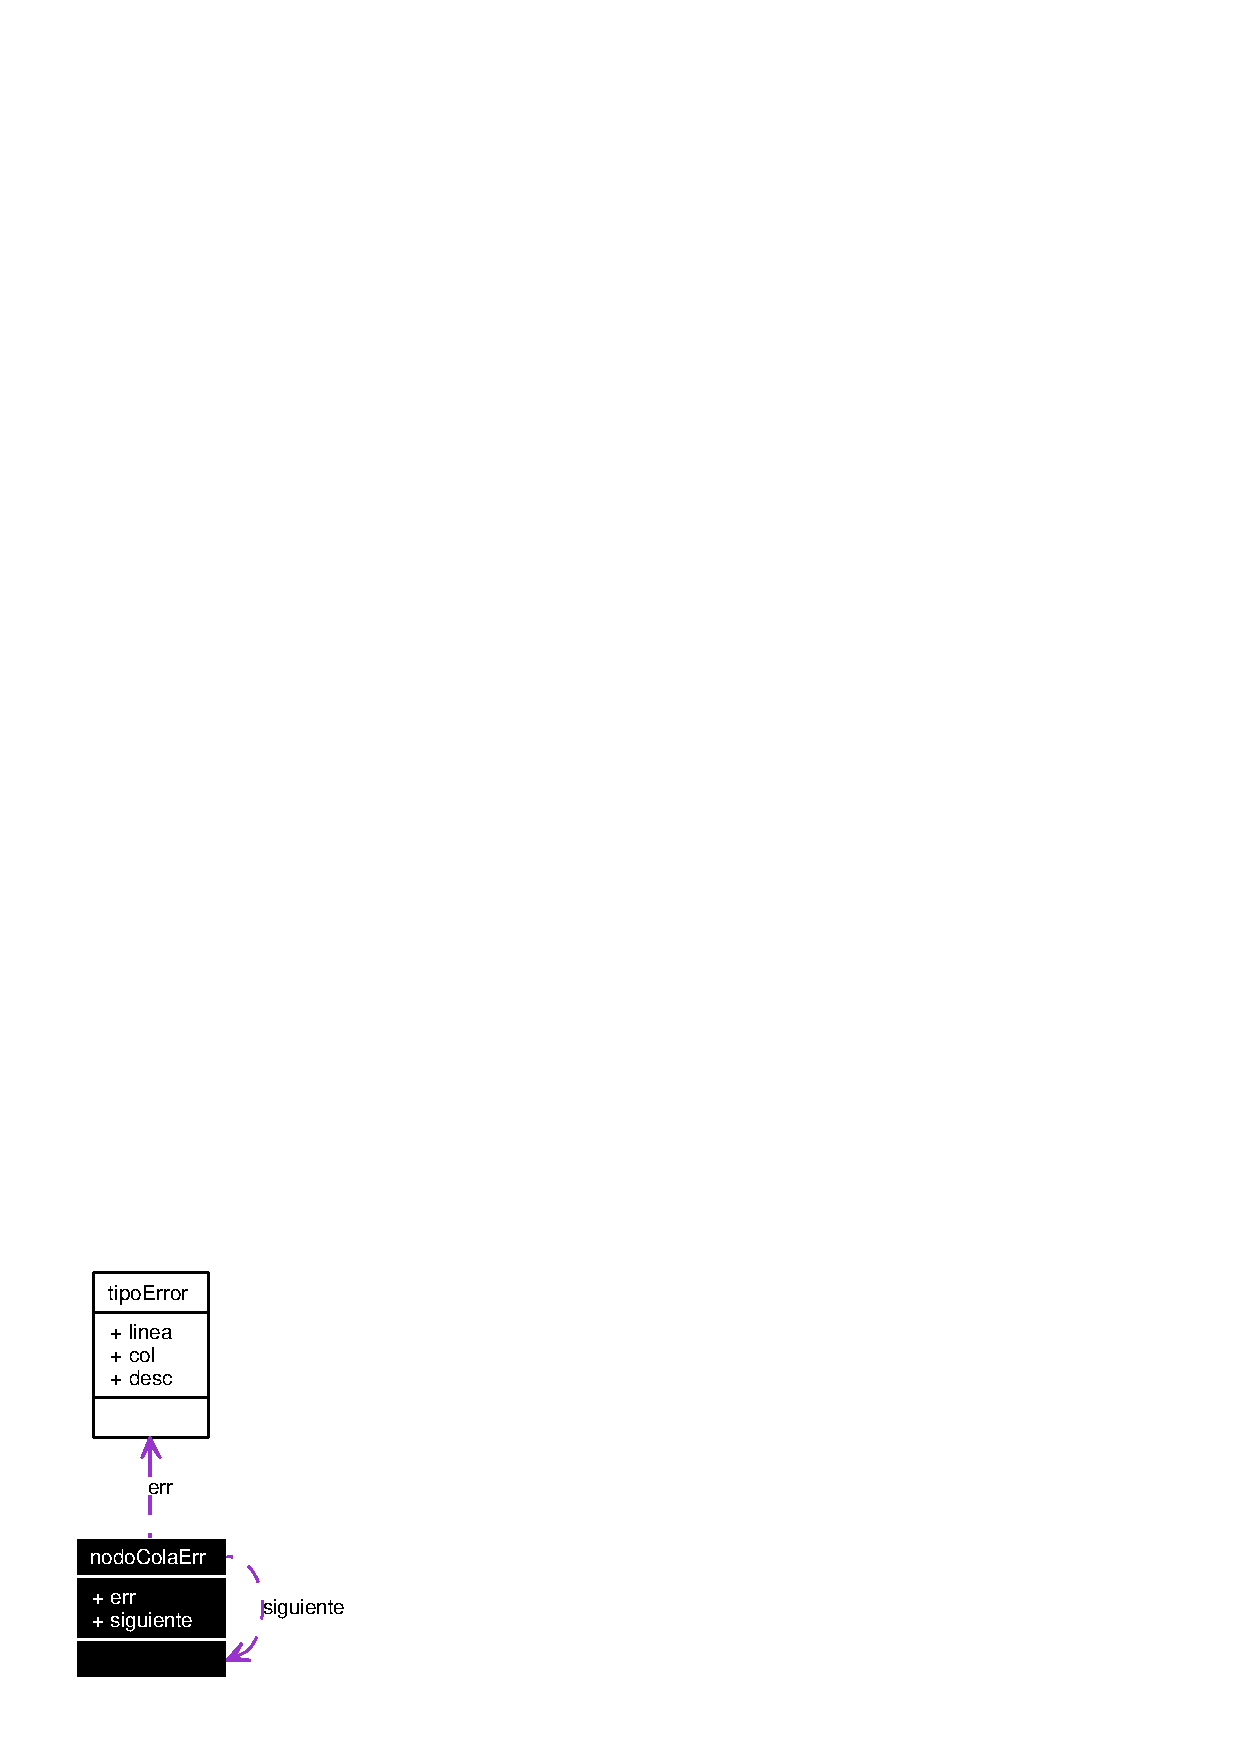
\includegraphics[width=83pt]{structnodoColaErr__coll__graph}
\end{center}
\end{figure}
\subsection*{Atributos p\'{u}blicos}
\begin{CompactItemize}
\item 
{\bf tipo\-Error} $\ast$ {\bf err}
\item 
{\bf nodo\-Cola\-Err} $\ast$ {\bf siguiente}
\end{CompactItemize}


\subsection{Descripci\'{o}n detallada}
Nodo de la cola de errores. 



Definici\'{o}n en la l\'{\i}nea 34 del archivo colaerr.h.

\subsection{Documentaci\'{o}n de los datos miembro}
\index{nodoColaErr@{nodo\-Cola\-Err}!err@{err}}
\index{err@{err}!nodoColaErr@{nodo\-Cola\-Err}}
\subsubsection{\setlength{\rightskip}{0pt plus 5cm}{\bf tipo\-Error}$\ast$ {\bf nodo\-Cola\-Err::err}}\label{structnodoColaErr_o0}




Definici\'{o}n en la l\'{\i}nea 35 del archivo colaerr.h.

Referenciado por encolar\-Error(), y sacar\-Error().\index{nodoColaErr@{nodo\-Cola\-Err}!siguiente@{siguiente}}
\index{siguiente@{siguiente}!nodoColaErr@{nodo\-Cola\-Err}}
\subsubsection{\setlength{\rightskip}{0pt plus 5cm}{\bf nodo\-Cola\-Err}$\ast$ {\bf nodo\-Cola\-Err::siguiente}}\label{structnodoColaErr_o1}




Definici\'{o}n en la l\'{\i}nea 36 del archivo colaerr.h.

Referenciado por encolar\-Error(), y sacar\-Error().

La documentaci\'{o}n para esta estructura fu\'{e} generada a partir del siguiente archivo:\begin{CompactItemize}
\item 
/media/docs/progra/c++/compiladores1/proy2/godzilla/src/{\bf colaerr.h}\end{CompactItemize}
